\section{Command-Muster}

\subsection{Problemstellung}
Es soll eine Universalfernbedienung entworfen werden. Hierbei k"onnen verschiedene Haushaltsger"ate angeschlossen werden. Die Fernbedienung soll f"ur jedes angeschlossene Ger"at einen An- und Ausschalter zur Verf"ugung stellen. Problem hierbei. Diverse Ger"atschaften besitzen haben unterschiedliche Schnittstellen. Bei manchen hei"sen diese schlicht und ergreifend anders als gefordert, bei anderen gibt es eine derart schlichte Kontrollfunktion nicht. Ein Beispiel w"are hier zum Beispiel ein Garagentor welches auf und zu gemacht werden kann aber auch eine Stereoanlage soll nicht nur angeschaltet werden, es soll auch ein Lied mit einer bestimmten Lautst"arke gespielt werden. 


\begin{figure}
	\centering
	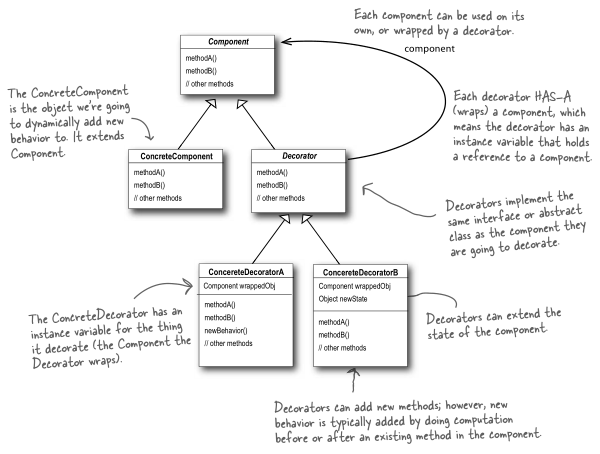
\includegraphics{decorator/img/decoratorUML}
	\caption{UML-Darstellung der zu implementierenden Fernsteuerung}
	\label{fig:commandRemote}
\end{figure}
